\chapter{Background}
\label{ch:background}
This chapter introduces and compares the monolithic software architecture and the microservice architecture. Further, benefits and challenges of the microservice architecture are outlined. Also, it introduces a well known and established use case notation technique and a standardized notation to capture business processes.



\section{Monolithic Software Architecture}
\label{sec:background:monolith}
The monolithic software architecture is a well-known and the most widely used pattern for Enterprise Applications, which usually are built in three main parts (top to bottom): The client-side user interface (Tier 3), the server-side application that contains the entire business logic (Tier 2) and the persistence layer handling the database access (Tier 1). Fig. \ref{fig:architekturMonolithVsMS} illustrates the architectural difference between a standard three tier application and a exemplary microservice-based architecture. The server-side application - \textit{the monolith} - is a single unit and deployed on one application server \cite{infoq}. The software structure, if well defined, is composed of self-contained modules (i.e. software components), where each module consists of a set of functions \cite{HeuristicsAlwis}.
The monolith implements a complex domain model, including all functions, many domain entities and their relationships.
For small applications, this approach works relatively well. They are simple to develop, test and deploy \cite{FunctionalDecompositionHeinrich}. Fast prototyping is supported by current frameworks and development environments (IDEs), which are still oriented around developing single applications \cite{infoq}.
\\
But once they grow in size, they become exceedingly difficult to understand and hard to maintain without reasonable effort \cite{FunctionalDecompositionHeinrich} \cite{ClassificationOfRefactoring}. A complex and large code base prevents a fast addition of new features and makes the application risky and expensive to evolve \cite{TowardsTechnique}.
Alterations to the system, even though they might be small, result in a redeployment of the whole monolith application due to its nature being a single unit \cite{FunctionalDecompositionHeinrich}. Moreover, it is difficult to adopt newer technologies without rewriting the whole application, as monoliths are build on a specific technology stack \cite{infoq} \cite{ExtractionMazlami}.\\
Scaling is only possible by duplicating the entire application, namely \textit{horizontal scaling}. Consequently, large portions of the infrastructure remain unused, if only parts of the application need to be upscaled or even used \cite{EnticeApproach} \cite{MigratingTowardsSurvey}. \\
Rui Chen describes the shortcomings of monolith as follows: "Successful applications
are always growing in size and will eventually become a
monstrous monolith after a few years. Once this happens,
disadvantages of the monolithic architecture will outweigh
its advantages" \cite{DataflowDrivenChen}.



\section{Microservices}
\label{sec:background:microservices}
M.Fowler and J.Lewis describe the microservice architectural style as "an approach to developing a single application as a suite of small services, each running in its own process and communicating with lightweight mechanisms, often an HTTP resource API"\cite{Fowler}.

\begin{figure}[t]
	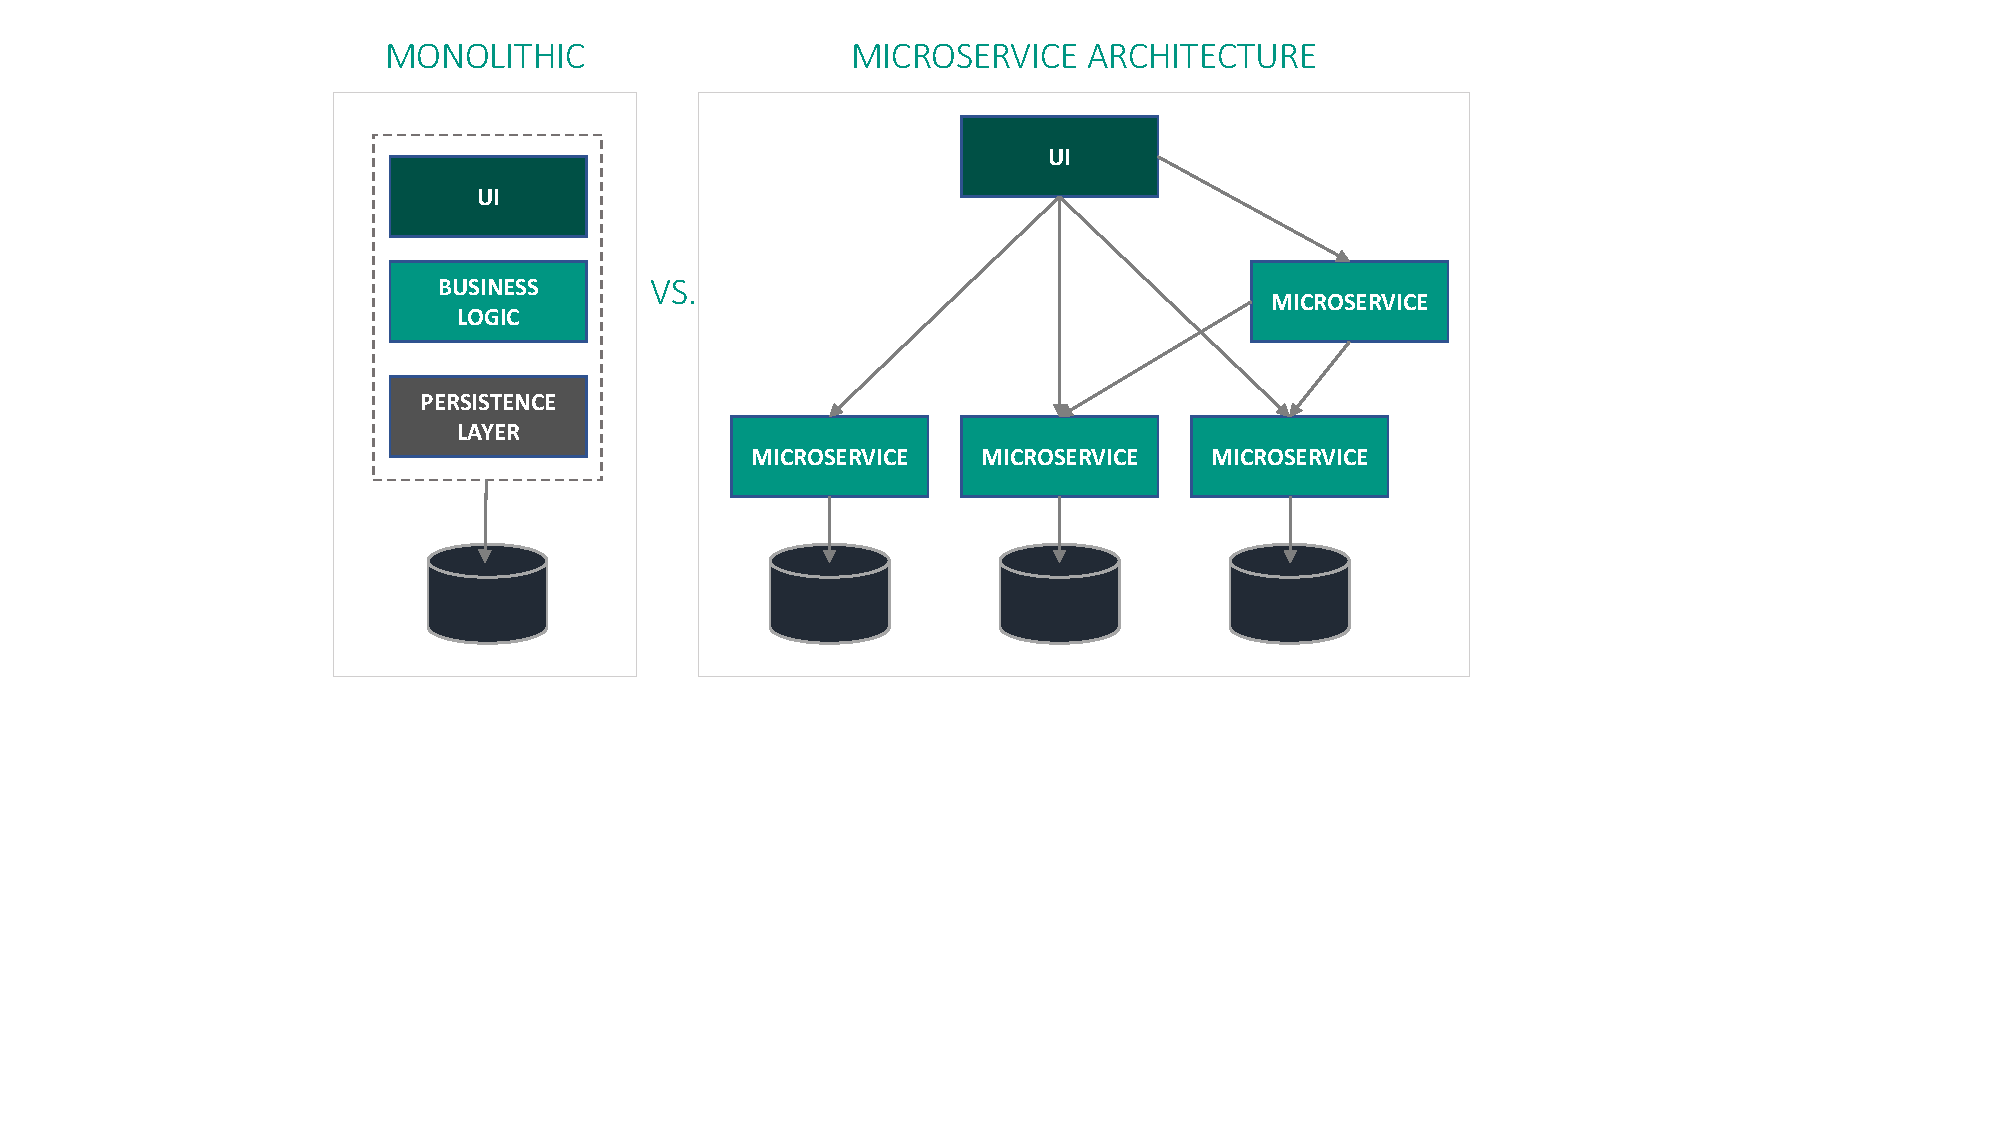
\includegraphics[width=\textwidth, trim={5cm 8cm 8cm 3cm}]{img/Architektur.pdf}
	\caption{Monolithic vs. Microservice Architecture}
	\label{fig:architekturMonolithVsMS}
\end{figure}

\subsection{Definition}
Yet, the term microservices is not formally defined in academia. A popular definition of microservices is  "a collection of cohesive and loosely coupled components, where each service implements a business capability"\cite{ObjectAwareAmiri}.
Amiri introduces three principles upon which the architecture is build: \textit{Bounded Context, Size, Independence} \cite{ObjectAwareAmiri}. \\
The first principle is about related functionality, that is combined in a single business capability - the  \textit{bounded context} \cite{FunctionalDecompositionHeinrich}. Each capability is implemented by one microservice. 
The \textit{Size} of a microservice is defined by the number of features it provides (namely bundled functional capabilities)  \cite{WorkloadbasedClustering}. There is no consensus about the "proper" size of a microservice \cite{DomainEngineeringMunezero}, but several guidelines exist: Services should focus on one business capability only \cite{ObjectAwareAmiri}. Others state, that the size of a microservice should not exceed a level, where it cannot be rewritten within six weeks \cite{WorkloadbasedClustering}. However, the sizes vary from system to system \cite{FunctionalDecompositionHeinrich} and even different sizes for each microservice in a specific system are possible \cite{DomainEngineeringMunezero}. The bottom line of \textit{Independence} is expressed in Amiri's description of microservices as "a collection of highly cohesive and loosely coupled components" \cite{ObjectAwareAmiri}. Highly cohesive services implement a relatively independent piece of business logic (at the most one business capability). Further, microservices should hardly depend on each other, which is the idea of being loosely coupled \cite{DataflowDrivenChen}.\\
Communication between microservices is achieved by lightweight message passing mechanisms such as \textit{REST}. Each service exposes a well defined interface (\textit{API}) with endpoints that provide information using standard data formats \cite{FunctionalDecompositionHeinrich}. 
The design of microservices mainly follows the \textit{Single Responsibility Principle (SRP)}: Each service should not have more than one reason to change \cite{TowardsUnderstandingEvolution}. The SRP mainly corresponds to the idea of not implementing more than one business capability.
The following paragraphs cover the benefits and challenges of the microservice architecture.





\FloatBarrier

\subsection{Benefits}
\textbf{Fast and Independent Deployment} \\
As a matter of fact, each microservice is deployed independently \cite{interfaceAnalysisBaresi}. Changes to the code do not result in a full redeployment of the entire application \cite{FunctionalDecompositionHeinrich}. Consequently, software developers are able to react much quicker to changes in business requirements. This includes an acceleration in error correction. Per contra, any changes in a monolithic code base require a time consuming build of a new version and the redeployment of the entire application \cite{Fowler}. \\

\noindent
\textbf{Availability, Resilience and Fault Isolation} \\
Microservices are designed to operate independently of each other and to tolerate failure of services \cite{Fowler}. Large parts of the application remain unaffected of partly failures and the availability of the system is, at least partly, guaranteed. Monolithic application do not provide this type of fault isolation. If a failure occurs, the whole application remains unavailable as it is usually running in a single process \cite{ExtractionMazlami}. \\
 
\noindent
\textbf{Scalability and Resource Utilisation} \\
Small and independent microservices allow more fine-granular horizontal scaling \cite{WorkloadbasedClustering}. Single services can be duplicated to cope with changing workload during runtime \cite{DataflowDrivenChen}. Thus, dynamic (de-)allocation of resources on demand prevent infrastructure from being idle \cite{HeuristicsAlwis}. Scaling monoliths can only be attained by duplicating the entire application, leaving resources unused \cite{ClassificationOfRefactoring}. Further, each microservice is deployed on the best suitable infrastructure for its needs, allowing a more efficient system organization \cite{infoq}. \\

\noindent
\textbf{Improved Productivity} \\
In traditional software development, teams are divided based on their expertise: Database architects, UI-developers and server-side engineers, resulting in a three-tiered application (cf. Sec.\ref{sec:background:monolith}). Additionally, software engineers are responsible for the development only. Deployment is part of the operations team. This team structure results in high communication overhead and slows down the productivity \cite{Mazlami}. \\
In contrast, microservices are organized around business capabilities and require cross-functional, independent teams \cite{ObjectAwareAmiri}. Each team has the full range of skills required for the end-to-end realization of a microservice, including UI-development, database architecture, back-end engineers and project management. 
This minimizes the need for communication and interaction between the teams and thus, speeds up the productivity. Ultimately, microservices enable a more agile flow of development and operation \cite{ClassificationOfRefactoring}, also referred as \textit{DevOps}. 
\\


\noindent
\textbf{Neutral development technology} \\
Microservices are highly decoupled from each other, as they use standardized and lightweight communication mechanisms such as REST \cite{FunctionalDecompositionHeinrich}. Microservices can be realized using different programming languages, technologies and even deployment environments \cite{DataflowDrivenChen}. Developers are consequently not longer limited to use a single technology for the whole application. They can choose the most appropriate technology for each particular business problem or try out some new technology without rewriting the whole application \cite{ServiceCutter} \cite{TowardsTechnique}. 
 



\subsection{Challenges}
The previous section provides a vast amount of benefits that come with microservices. However, microservices are not the panacea of software engineering. System developers have to face challenges that can mitigate the benefits as described previously. The challenges are described in the following. \\ 

\noindent
\textbf{Expensive Communication}\\
Microservice use network protocols such as \textit{HTTP} to communicate with each other. Compared to standard inter process communication (\textit{IPC}) as used in monoliths, remote procedure calls a more expensive \cite{SystematicMappingStudyMicroservice}. As a consequence, applications experience a decrease in performance as network communication is generally slower than \textit{IPC}.\\

\noindent
\textbf{Technical Challenges}\\
Microservices require a high degree of infrastructure automation \cite{MigratingTowardsSurvey}. The benefits of fast and independent deployment cannot be utilized, if it has to be done manually. Dynamic (de-)allocation of resources when scaling individual microservices need a well defined and structured cloud environment \cite{MigratingCloud}. 
Besides, the distributed microservice landscape complicates the logging mechanisms and performance monitoring \cite{SystematicMappingStudyMicroservice}. Traditional centralized logging, as it is used in monolithic applications, is not longer applicable. Instead, a careful aggregation system to gather logging and monitoring data from each service is required.\\

\noindent
\textbf{Organizational Challenges}\\
The microservice approach needs the establishment of cross-functional teams \cite{Fowler}. Adopting \textit{Continuous Practices}, such as \textit{Continuous Deployment}, are essential for the success of a profitable microservice architecture. Therefore, closer collaboration between development teams, operational staff and management has to be established. In summary, a costly and time consuming restructuring process of the entire organization is required \cite{NikoProseminar}. \\



\noindent
\textbf{Data Consistency}\\
Distributed systems need to share data. Heinrich \textit{et al.} propose two concepts for the database architecture \cite{FunctionalDecompositionHeinrich}: The first concept applies the basic idea of the microservice approach, as it splits the database into several parts. Each microservice has its own database which manages the entities that belong to the corresponding bounded context. Higher speed and horizontal scaling are facing data consistency issues. Data needs to be synchronized which leads to inconsistency, if services are unavailable. The second concept is about sharing a single database. On the one hand, this approach overcomes the issue of consistency, as data is stored centrally. On the other hand, sharing results in a loss of independence. Scaling can only be achieved through replicating the whole database. According to Tyszberowicz \textit{et al.}, the first concept is preferred \cite{FunctionalDecompositionHeinrich}. \\



\noindent
\textbf{Decomposition}\\
Decomposing a system into microservices is a very complex task that requires experienced system architects and domain experts \cite{Fowler}. It is irrelevant whether an existing system is decomposed into microservices or whether a new system is designed as a microservice-based application. The effort is very high in both cases.\\
Identifying the right granularity of microservice is one of the key issues. Too fine grained services cause inefficiency due to a high amount of expensive inter-service calls \cite{DomainEngineeringMunezero}. On the other hand, too coarse grained microservices debilitate the scalability. \\

 



\section{Use Cases}
\label{sec:PrepApproach:UC}
Use Cases are a widely adopted technique to document software system requirements. Generally, they describe the interaction between actors (usually system users) and the software system itself. In this thesis, use cases are provided as semi-structured tables (following the notation presented by Cockburn \textit{et al.} \cite{Cockburn}). \\ An example is given in Table \ref{tab:exampleUseCase}: Each use case has a unique identifier and a short description, followed by necessary preconditions and a trigger that causes the execution. The standard process is the main part and describes the success steps of the Use Case. Extensions provide additional information like alternatives or exceptional processes that occur in case of an unsuccessful step. 




\begin{table}[!h]
	\centering
	\begin{tabularx}{\textwidth}{|l||X|}
		\hline
		UC 5 & Show Stock Reports \\ 
		\hline
		Brief Description &  The opportunity to generate stock-related reports is provided
		by the Trading System. \\
		\hline
		Precondition & The reporting GUI at the Store Client has been started. \\
		\hline
		Trigger & The Store Manager wants to see statistics about his store. \\
		\hline
		Postcondition & The report for the Store has been generated and is displayed on
		the reporting GUI. \\
		\hline 
		Standard Process &
		
		1. The Store Manager enters the store identifier and presses the button Create
		Report.  \\
		& 2. A report including all available stock items in the store is displayed. \\  
		\hline
		Extensions & (none) \\ \hline
		
		
	\end{tabularx}
	\caption{Example Use Case in Tabular Form, Source: \cite{CoCoMEOld}}
	\label{tab:exampleUseCase}
	
\end{table}

\noindent
Besides being a widely adopted technique to specify system requirements, the textual use case notation is understandable without further technical knowledge. Neither previous knowledge in specific graphic notations like UML, nor the capability to create a complex domain model is necessary. Consequently, all sorts of stakeholders (non-technical and technically experienced) are capable to provide the necessary information in terms of use cases. \\
However, the transformation into business models as presented in Sec.\ref{sec:PrepApproach:TransformUCtoBPMN} is not always trivial and requires some manual effort to produce high quality business processes. Nevertheless, it is necessary as the system requirements of the running example are given in form of textual use cases.





\section{Business Process and Model Notation}
\label{sec:PrepApproach:BPMN}
The Business Process and Model Notation (BPMN) is a graph oriented language to describe business processes. Originally, BPMN was designed to describe activities and their control flow dependencies only \cite{VisualizeBPMN}. Since the introduction of BPMN 2.0, it is possible to model the data needs and the data results of activities \cite{OMG}. Consequently, BPMN is capable of expressing the control flow and to approximate the data flow of business processes \cite{DataFlowErrorBPMN}. In the remainder, BPMN and BPMN 2.0 is used interchangeably. \\
BPMN is easy-to-use, powerful and widely adopted in academia and industry. Hence, BPMN is a suitable approach to extract the implicitly given data flow and control flow in the use case description. Sec.\ref{sec:PrepApproach:TransformUCtoBPMN} introduces a formal approach to generate BPMN processes from use case sets. Next, the BPMN 2.0 process definition is shortly introduced:

%"l, b, r, t"
\begin{figure}[h!]
	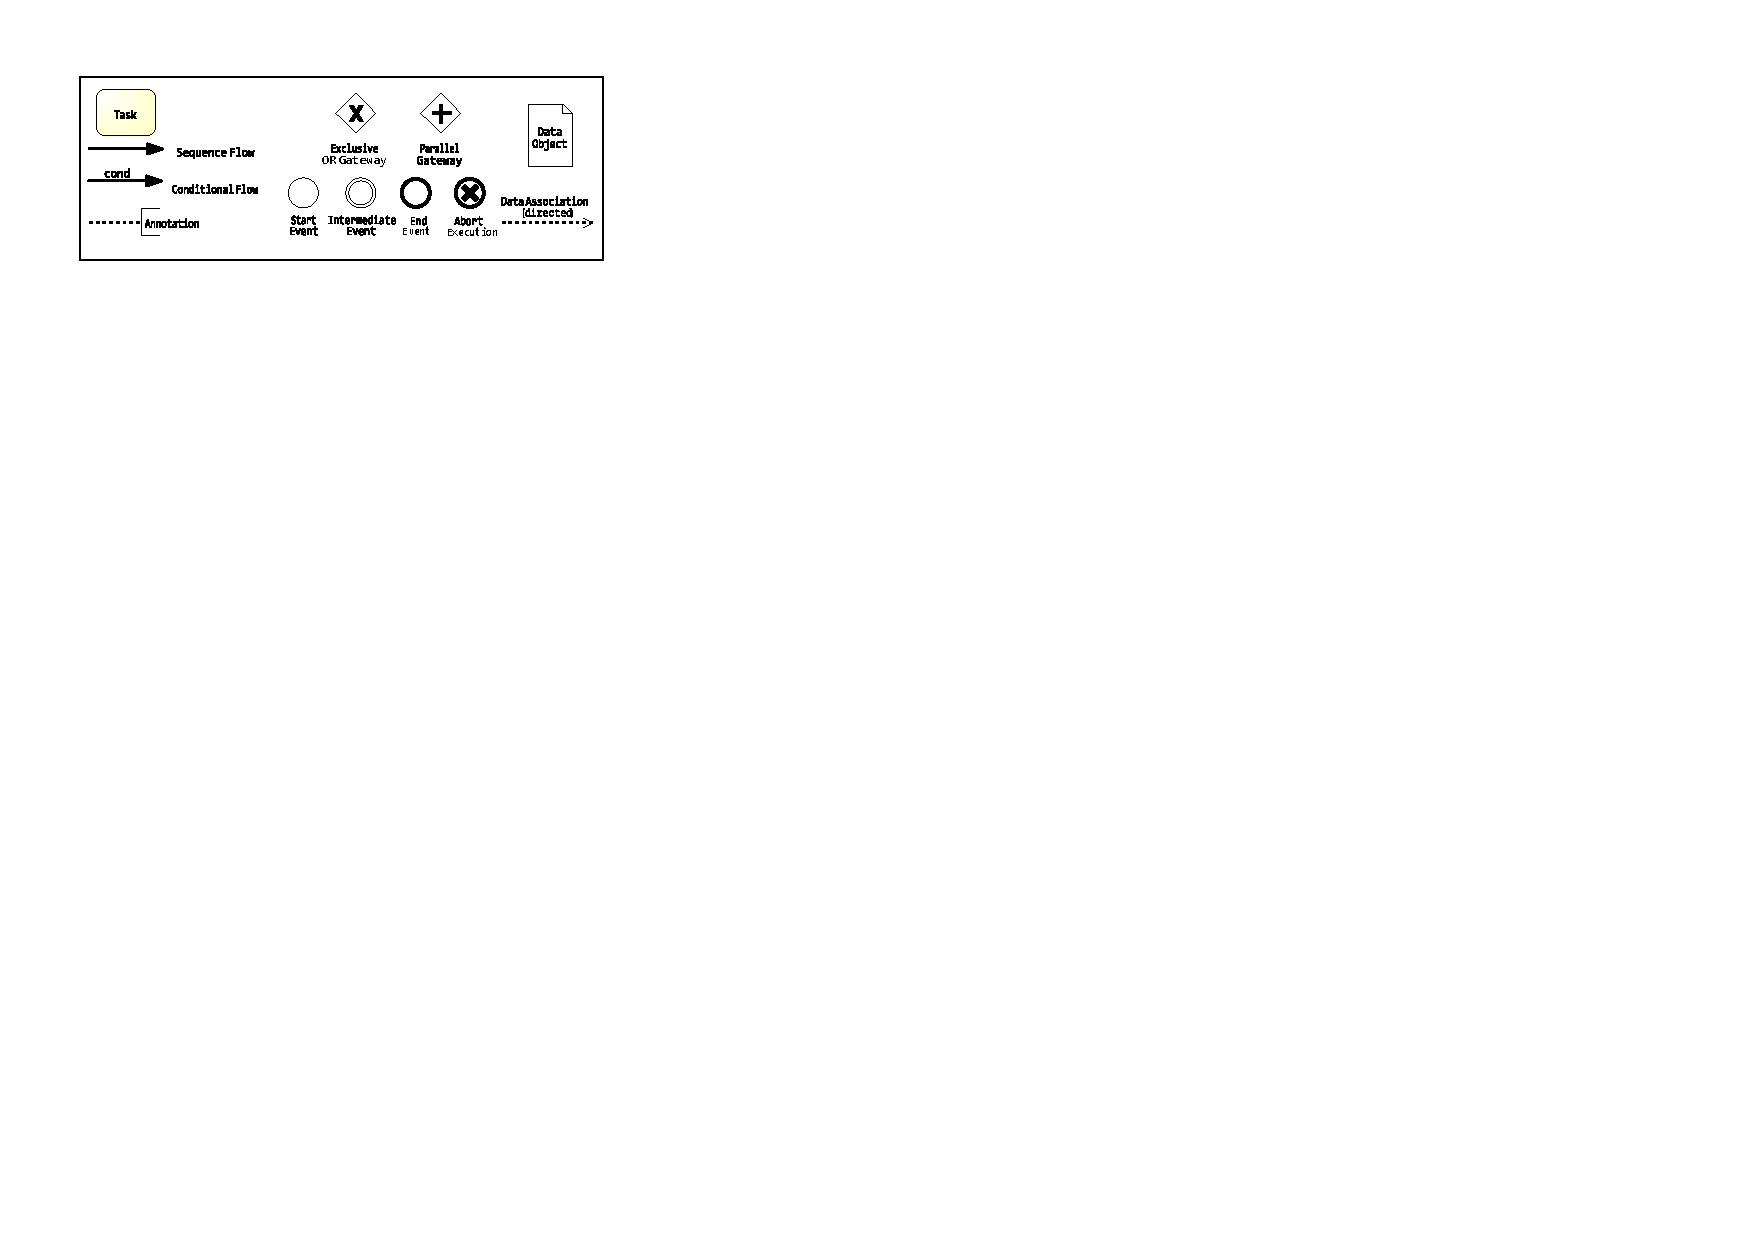
\includegraphics[width=\textwidth, trim={1cm 16.8cm 19.5cm 1cm}]{img/Overview.pdf}
	\caption{BPMN Notation (Subset)}
	\label{fig:BPMNSubset}
\end{figure}

\noindent
Fig.\ref{fig:BPMNSubset} shows the subset of BPMN symbols, that is required for the approach presented in this thesis\footnote{The entire specification is available at https://www.omg.org/spec/BPMN/2.0/}. Control flow activities are modelled as atomic \textit{Tasks} and connected through \textit{Sequence Flow Arcs}. \textit{Conditional Flow Arcs} integrate decision points into the control flow. Navigation decisions are based on the conditions related to the individual arcs. Such decision point are the \textit{Exclusive Or Gateway} and the \textit{Parallel Gateway}. Regarding the first gateway, if one of the incoming flows is triggered exactly one outgoing flow is activated based on the condition. For the latter, all outgoing flows are activated as soon as all of its incoming flows are activated. Each BPMN process starts with a \textit{Start Event} and ends with an \textit{End Event}. In case of several branches (due to Gateways) stop events need to be placed at each end. \textit{Intermediate Events} mark any other event that occurs during the process. The trigger for an event is modelled using the \textit{Annotation} symbol. The \textit{Abort Execution Event} extend the \textit{End Event} and marks the error-prone end of a business process. \\
When it comes to data, each \textit{Task} may or may not require and/or produce data. Directed \textit{Data Association Arcs} provide the opportunity to model data needs and data results. In case a task requires data, the corresponding \textit{Data Objects} are connected to the task with the arrowhead attached to the task, whereas producing data works in the opposite direction. \\








